\documentclass[final]{beamer}

% ====================
% Packages
% ====================

\usepackage[T1]{fontenc}
\usepackage{lmodern}
\usepackage[size=a0,scale=1.2]{beamerposter}
\usetheme{gemini}
\usecolortheme{UNR}
\usepackage{graphicx}
\usepackage{booktabs}
\usepackage{svg}
\usepackage{pgfplots}
\usepackage{lipsum}
\usepackage{geometry}
\geometry{paperwidth=48in, paperheight=36in}


% ====================
% Lengths
% ====================

% If you have N columns, choose \sepwidth and \colwidth such that
% (N+1)*\sepwidth + N*\colwidth = \paperwidth
\newlength{\sepwidth}
\newlength{\colwidth}
\setlength{\sepwidth}{0.025\paperwidth}
\setlength{\colwidth}{0.3\paperwidth}

\newcommand{\separatorcolumn}{\begin{column}{\sepwidth}\end{column}}

% ====================
% Title
% ====================

\title{DeadDrop}

\author{Jann Arellano, Brian Buslon\\Keaton Clark, Lloyd Gonzales}

\institute[shortinst]{CSE Department, UNR \\ \textbf{Advisor:} Shamik Sengupta. Professor. University of Nevada, Reno \\ \textbf{Instructors:} David Feil-Seifer, Devrin Lee, Sara Davis}

% remove this section if poster is for inhouse project
\addtobeamertemplate{headline}{} 
{
    \begin{tikzpicture}[remember picture,overlay]
    % tweak these sizes according to the logo of the company:
    % xshift, yshift, height
    \node [anchor=north west, inner sep=3cm] at ([xshift=-1.5cm,yshift=2cm]current page.north west)     {
\includegraphics[height=12cm]{images/unr.png}}; 
    \end{tikzpicture} 
}

% ====================
% Body
% ====================

\begin{document}


\begin{frame}[t]
\begin{columns}[t]
\separatorcolumn

\begin{column}{\colwidth}

  \begin{alertblock}{Abstract}
    \it{
      DeadDrop is a command and control (C2) framework used for cybersecurity activities such as post-exploitation operations and penetration testing.
      Penetration testing is where security professionals identify weaknesses in an organization's network.
      Using a C2 framework in testing greatly benefits security engineers, as they can identify security weaknesses through the reporting and logging functionalities provided by the C2 framework.
      However, unlike existing frameworks, DeadDrop focuses on leveraging features in trusted websites such as YouTube and Craigslist to communicate with agents and exfiltrate data, masking its activity within the noise of popular websites.
      By abusing the "trust" associated with large, well-known services, DeadDrop provides security engineers with new insights into identifying covert attack techniques and exploits.
    }
  \end{alertblock}

  \begin{block}{User Interface}
    
    The user interface is built with Svelte and is served by a Django backend.
    The user is able to interact with all of the features provided by the backend and the agents.

    \begin{figure}
      \centering
      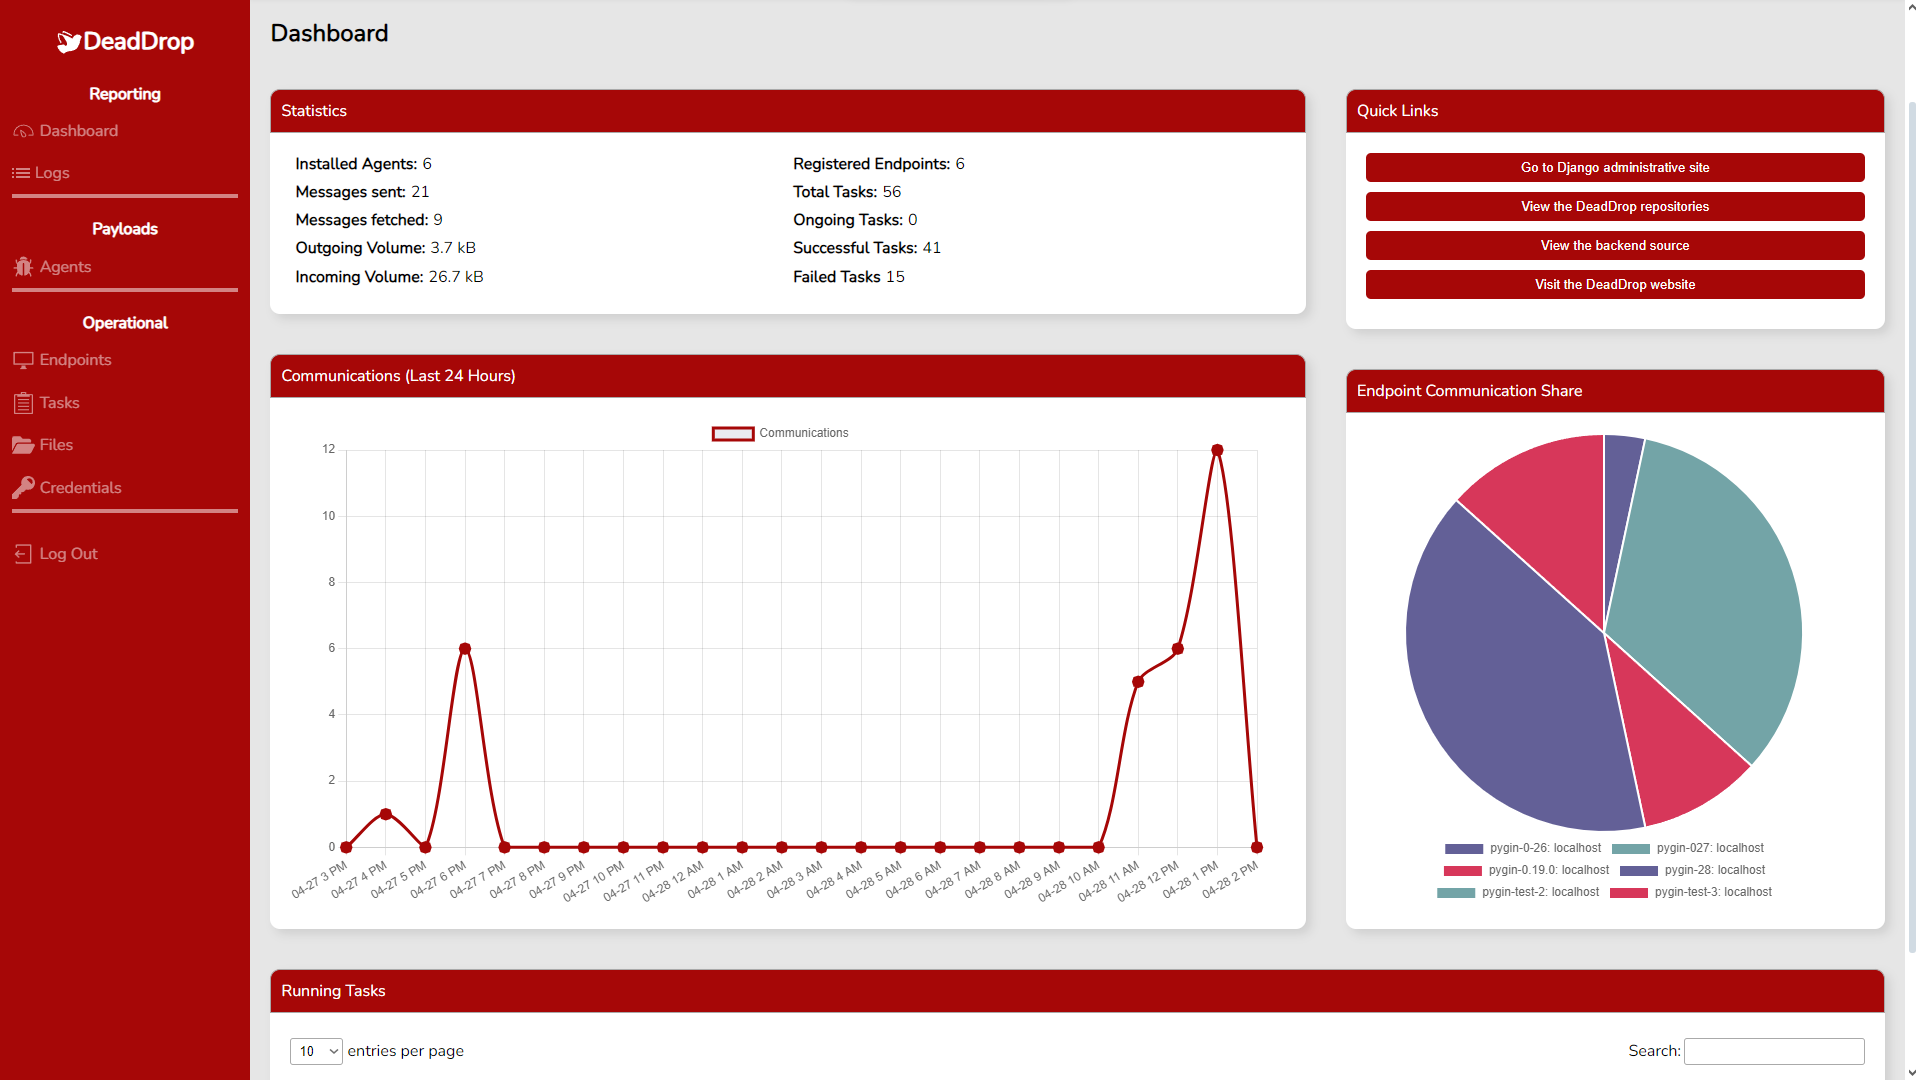
\includegraphics[width=\textwidth]{images/frontend.png}
      \caption{\quad UI built with Svelte}
      \label{fig:frontend}
    \end{figure}

  \end{block}

  \begin{block}{Future Work}

    \heading{Near Future}
      \begin{itemize}
        \item Server log and act on heartbeat messages
        \item Implement credential/file imports from command results
        \item Implement log bundle support
        \item Implement the guardrail system
        \item Implement sitewide search
      \end{itemize}
    \heading{Far Future}
      \begin{itemize}
        \item Github Actions auto generate releases
        \item Full PyInstaller support (Windows)
        \item Implement killswitch command
        \item Pygin uninstall on server deletion
      \end{itemize}
  \end{block}


\end{column}

\separatorcolumn

\begin{column}{\colwidth}

  \begin{block}{Project Overview}

    Like many C2 frameworks, DeadDrop provides the following major features through its web interface and internal APIs:

    \begin{itemize}
      \item \textbf{Payload Generation:}
        Users can build and configure new instances of agents, leveraging containers to allow platform-agnostic building.
      \item \textbf{Messaging:}
        Users can communicate with agents to execute commands on remote devices and receive results.
      \item \textbf{Reporting and administration:}
        The server provides permissions systems and logging for developing organizational reports and ensuring accountability.
    \end{itemize}

  \end{block}

  \begin{block}{Architecture}

    At the highest level, DeadDrop follows a client-server model, shown in figure \ref{fig:arch}, whereby a single attacker-controlled server interacts with one or more agents (clients) installed on remote machines via an arbitrary medium. 
    Each agent is platform-specific and may support different functionality, but must implement certain basic features shared between all agents regardless of implementation language or target platform. 

    \begin{figure}
      \centering
      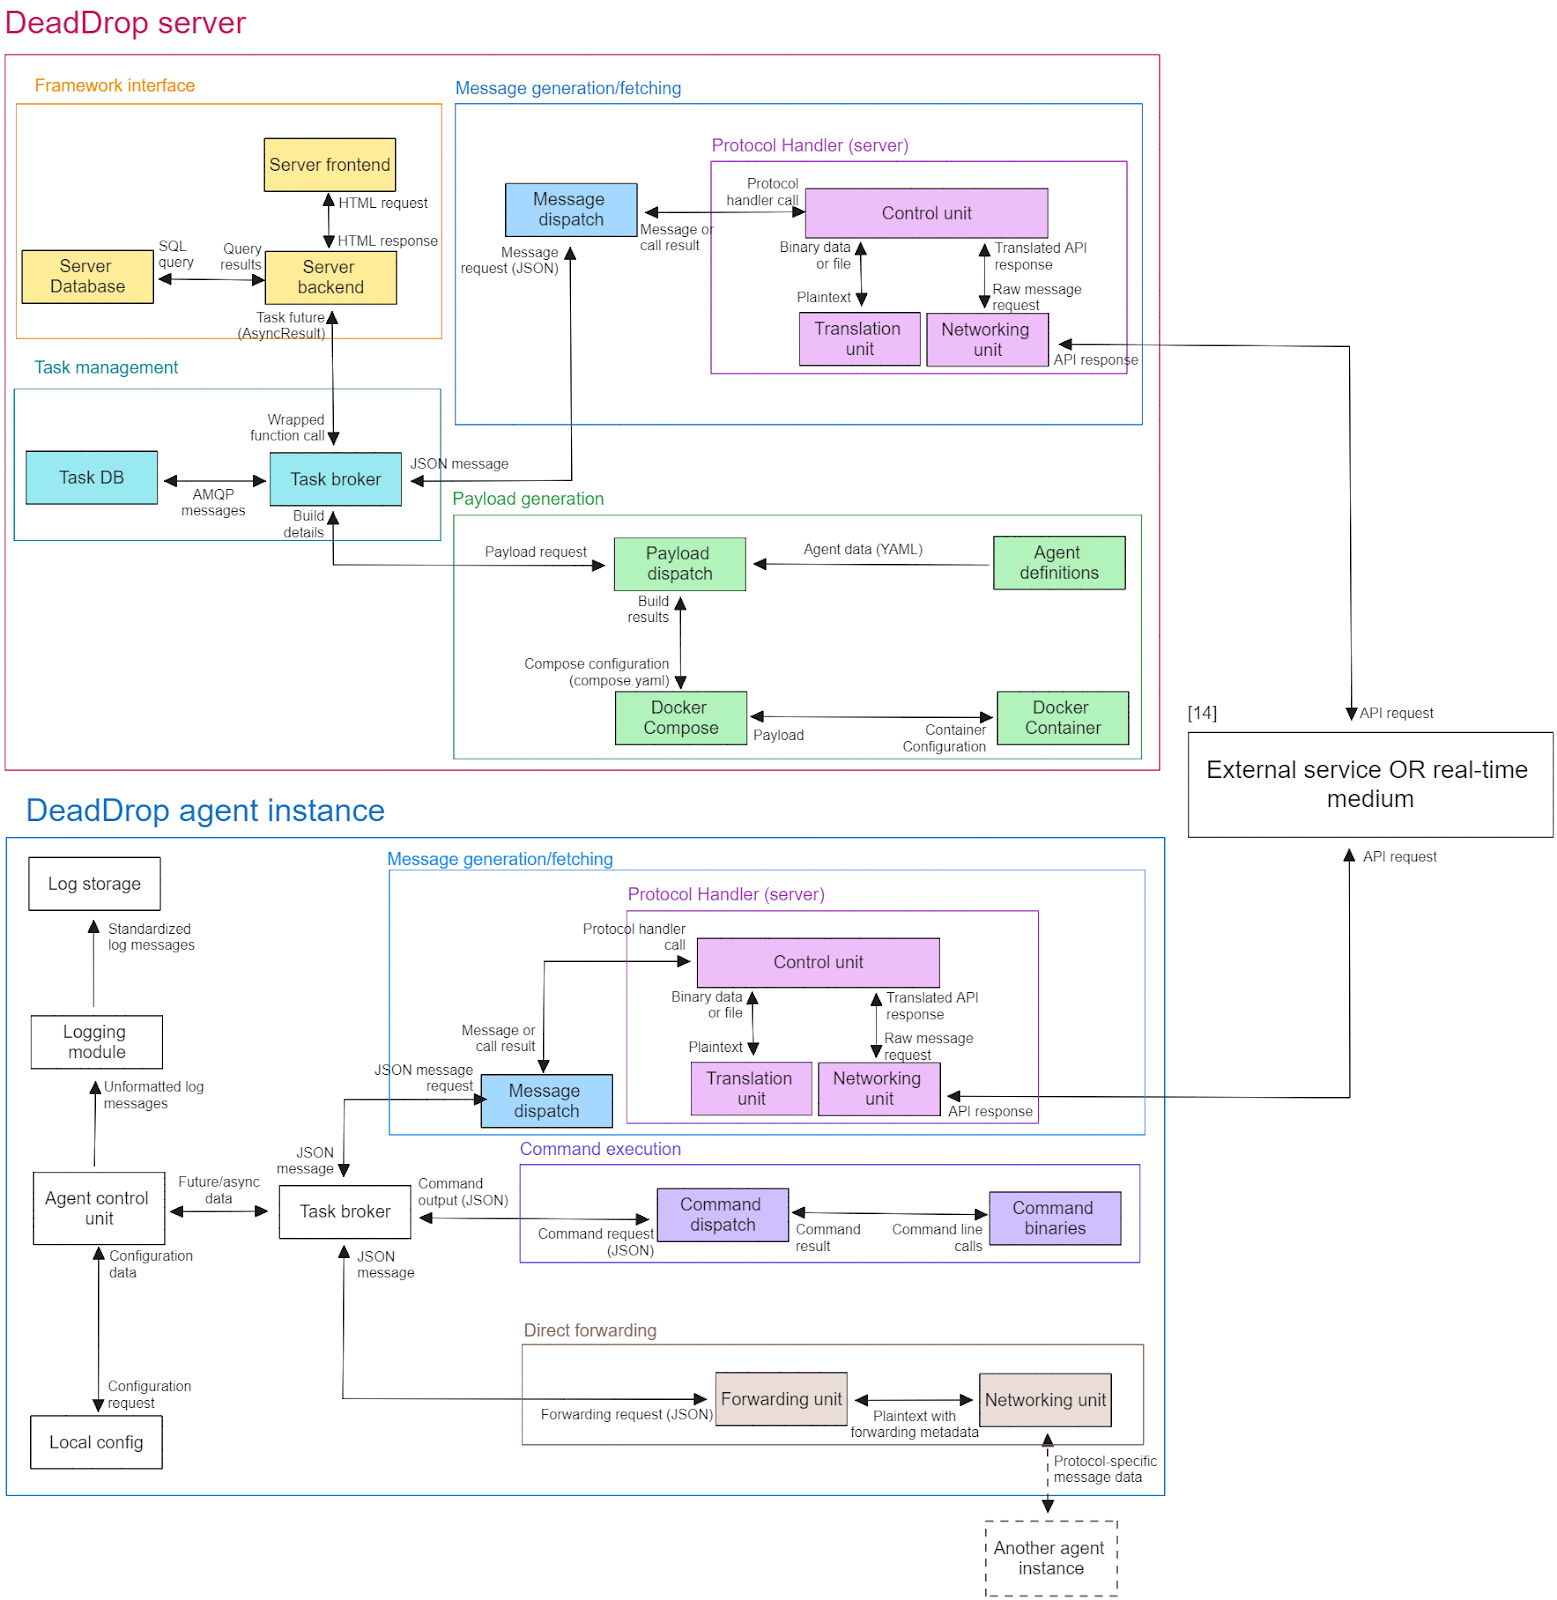
\includegraphics[width=\textwidth]{images/architecture.png}
      \caption{\quad A high-level overview of DeadDrop’s (non-object-oriented) architectural pattern}
      \label{fig:arch}
    \end{figure}

  \end{block}
  \begin{block}{}
    
    \it{This project was developed in Spring 2024 as part of the course CS 426 Senior Projects in Computer Science}

  \end{block}

\end{column}

\separatorcolumn

\begin{column}{\colwidth}

  \begin{block}{Communication Protocols}
    The communication protocols are the abstract definitions and formal implementations for communicating over legitimate. Functionally, communication protocols are independent of any particular agent.
    That is, they serve as an opaque layer that can be seen by any agent as a very delayed but reliable form of TCP, and does not depend on a particular agent’s features to operate.
    They support end-to-end encryption and define a procedure for coordinating the encryption key between the server and the agent.
    They define a procedure coordinating the website and specific service used, as well as how to handle delays, out-of-order messages, or lost messages. For example, if YouTube is used as a communication channel, the server might “drop” new commands as comments on a video uploaded to a specific channel agreed upon by the server and agent ahead of time.
    Currently we have a video/YouTube protocol as well as a Craigslist protocol.

    \begin{figure}
      \centering
      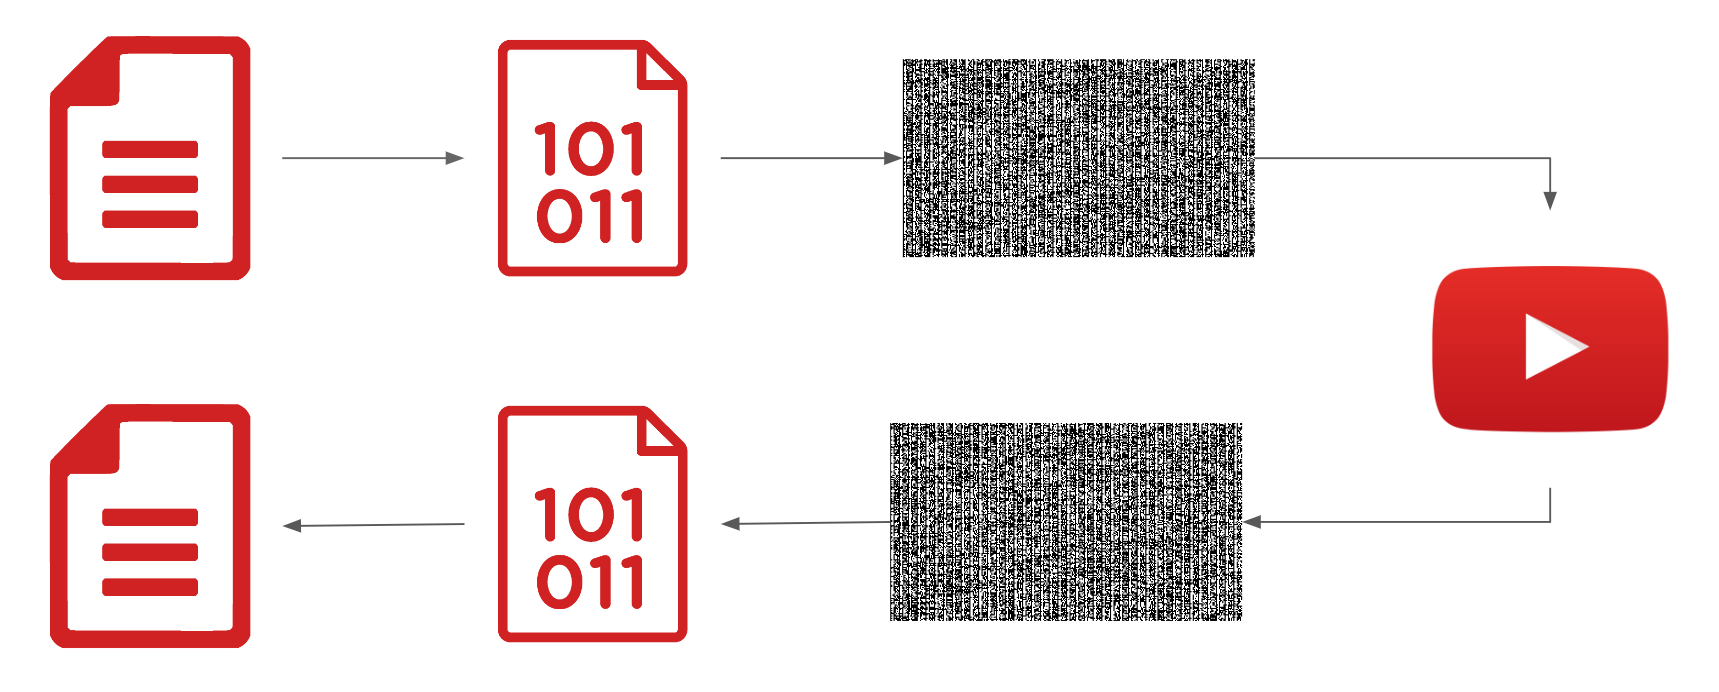
\includegraphics[width=\textwidth]{images/encode.png}
      \caption{\quad Example of a message transmission through YouTube}
      \label{fig:encode}
    \end{figure}
    Figure \ref{fig:encode} demonstrates how an agent can transmit data back to the server. 
    A text file is re-interpreted as a binary file and encoded in the frames of a video (white pixels are 1's and black pixels are 0's). 
    This video can then be uploaded to YouTube where the server can pull it down, reverse the algorithm to encode the video to transform it back into binary, and then convert it back to a text file.
  \end{block}
  \begin{block}{Conclusion}

    A brief summary of major accomplishments includes:
    \begin{itemize}
      \item
        The implementation of a package manager, allowing users to build, distribute, and install multiple agents in individual DeadDrop installations;
      \item
        The development of standardized metadata files that allow agents to expose important interfaces and information in a language-agnostic manner;
      \item
        The publishing of a meta-library for DeadDrop, providing common interfaces and expectations for agents, messages, and other core data structures;
      \item
        Continued research and development toward adapting the YouTube communication protocol to operate over live Zoom calls, in addition to a new architecture and a mock YouTube service;
      \item
        New research towards operating a communication protocol over Slack and Facebook Marketplace;
      \item
        Continued progress towards a more robust authentication and user system, allowing proper logging and accountability for actions taken through the framework; and
      \item
        The use of Docker Compose on all major components (the server, the frontend, and Pygin), which reduces setup time on individual machines and increases overall reliability.
    \end{itemize}


  \end{block}

  %\begin{block}{References}
  %  \nocite{*}
  %  \footnotesize{\bibliographystyle{plain}\bibliography{poster}}
  %\end{block}
  

\end{column}

\separatorcolumn
\end{columns}
\end{frame}

\end{document}
